\documentclass[11pt]{article}
\usepackage[utf8]{inputenc}
\usepackage[T1]{fontenc}
\usepackage{lmodern}
\usepackage{geometry}
\usepackage{microtype}
\usepackage{xcolor}
\usepackage{booktabs}
\usepackage{graphicx}
\usepackage{caption}
\usepackage{hyperref}
\geometry{margin=1in}
\graphicspath{{../report/figures/}{report/figures/}}
\hypersetup{
    colorlinks=true,
    linkcolor=blue,
    urlcolor=blue,
    citecolor=blue
}
\setlength{\parskip}{0.65em}
\setlength{\parindent}{0pt}

\title{\textbf{Executive Summary}\\
\large AI-Driven Data Research in Quantitative Finance}
\author{
CHAN Ho Lam \quad CHOI Man Hou \quad TSOI Ching Yi\\
\small IEDA4920 Final Year Project \\
\small HKUST \quad WorldQuant Consulting (Beijing) Co., Ltd.
}
\date{April 2026}

\begin{document}
\maketitle

\section*{Project Overview}

This executive summary presents the IEDA4920 Final Year Project,
\textit{AI-Driven Data Research in Quantitative Finance}. The project develops
an end-to-end framework that converts SEC Item 1A \textit{Risk Factors}
disclosures into hierarchical textual-risk exposures, semantic peer networks,
topology-only ST-GAT forecasts, econometric diagnostics, and academic
portfolio-backtesting outputs.

Annual 10-K risk paragraphs are extracted from EDGAR filings, mapped into a
dynamic macro-meso taxonomy, aggregated into firm-year exposure vectors, and
converted into annual semantic peer graphs. These graphs are used to test
whether disclosure-implied peer topology improves one-year-ahead return and
volatility forecasts beyond each firm's own financial and market features.

\section*{Core Research Contribution}

The central modeling contribution is a strict graph-topology ablation. The full
ST-GAT model uses
\[
    A_t = I + A_{risk,t},
\]
while the identity baseline uses
\[
    A_t = I.
\]
This design isolates the incremental value of textual-risk peer topology. If
the full graph improves over the identity baseline, the gain is attributable to
semantic peer links rather than to a different feature set or a weaker model
family.

\section*{Empirical Design}

The forecasting panel covers risk years 2006--2024. The chronological split is:

\begin{center}
\begin{tabular}{@{}lll@{}}
\toprule
Stage & Years & Role \\
\midrule
Training & 2006--2016 & Model fitting, feature scaling, and imputation statistics \\
Validation & 2017--2020 & Hyperparameter selection and early-stopping signal \\
OOS review panel & 2021--2024 & Final forecast and portfolio diagnostics \\
\bottomrule
\end{tabular}
\end{center}

Each firm-year node uses 12 backward-looking financial and market features,
standardized using training-year statistics only. Features and risk topology
are aligned to the July-to-June feature window, while forward return and
volatility targets are measured over the following July-to-June window.

\section*{Main Verified Results}

The finalized report is conservative about the default Meso graph evidence.
On the exported 2021--2024 OOS review panel, the default Meso ST-GAT improves
return MAE and return rank, but not averaged OOS RMSE. A full-window
\texttt{theta040} taxonomy sensitivity run provides stronger forecast-error
evidence:

\begin{center}
\begin{tabular}{@{}lll@{}}
\toprule
Metric & Identity baseline & ST-GAT \\
\midrule
Averaged RMSE (\texttt{theta040}) & 0.3523 & 0.3176 \\
Averaged MAE (\texttt{theta040}) & 0.2546 & 0.2012 \\
Averaged Spearman rank (\texttt{theta040}) & -0.0403 & 0.1055 \\
Volatility RMSE (\texttt{theta040}) & 0.2082 & 0.1555 \\
Default return Spearman rank & 0.1564 & 0.1650 \\
\bottomrule
\end{tabular}
\end{center}

The clearest improvement is in volatility forecasting under \texttt{theta040}.
Paired Macro-level runs are much denser but underperform identity baselines,
so the report interprets the result as selective Meso information transfer
rather than a generic benefit from broad category coverage. The default taxonomy
remains useful as a conservative baseline because it shows that graph gains are
not automatic and must be sensitivity-tested.

\begin{figure}[!htbp]
    \centering
    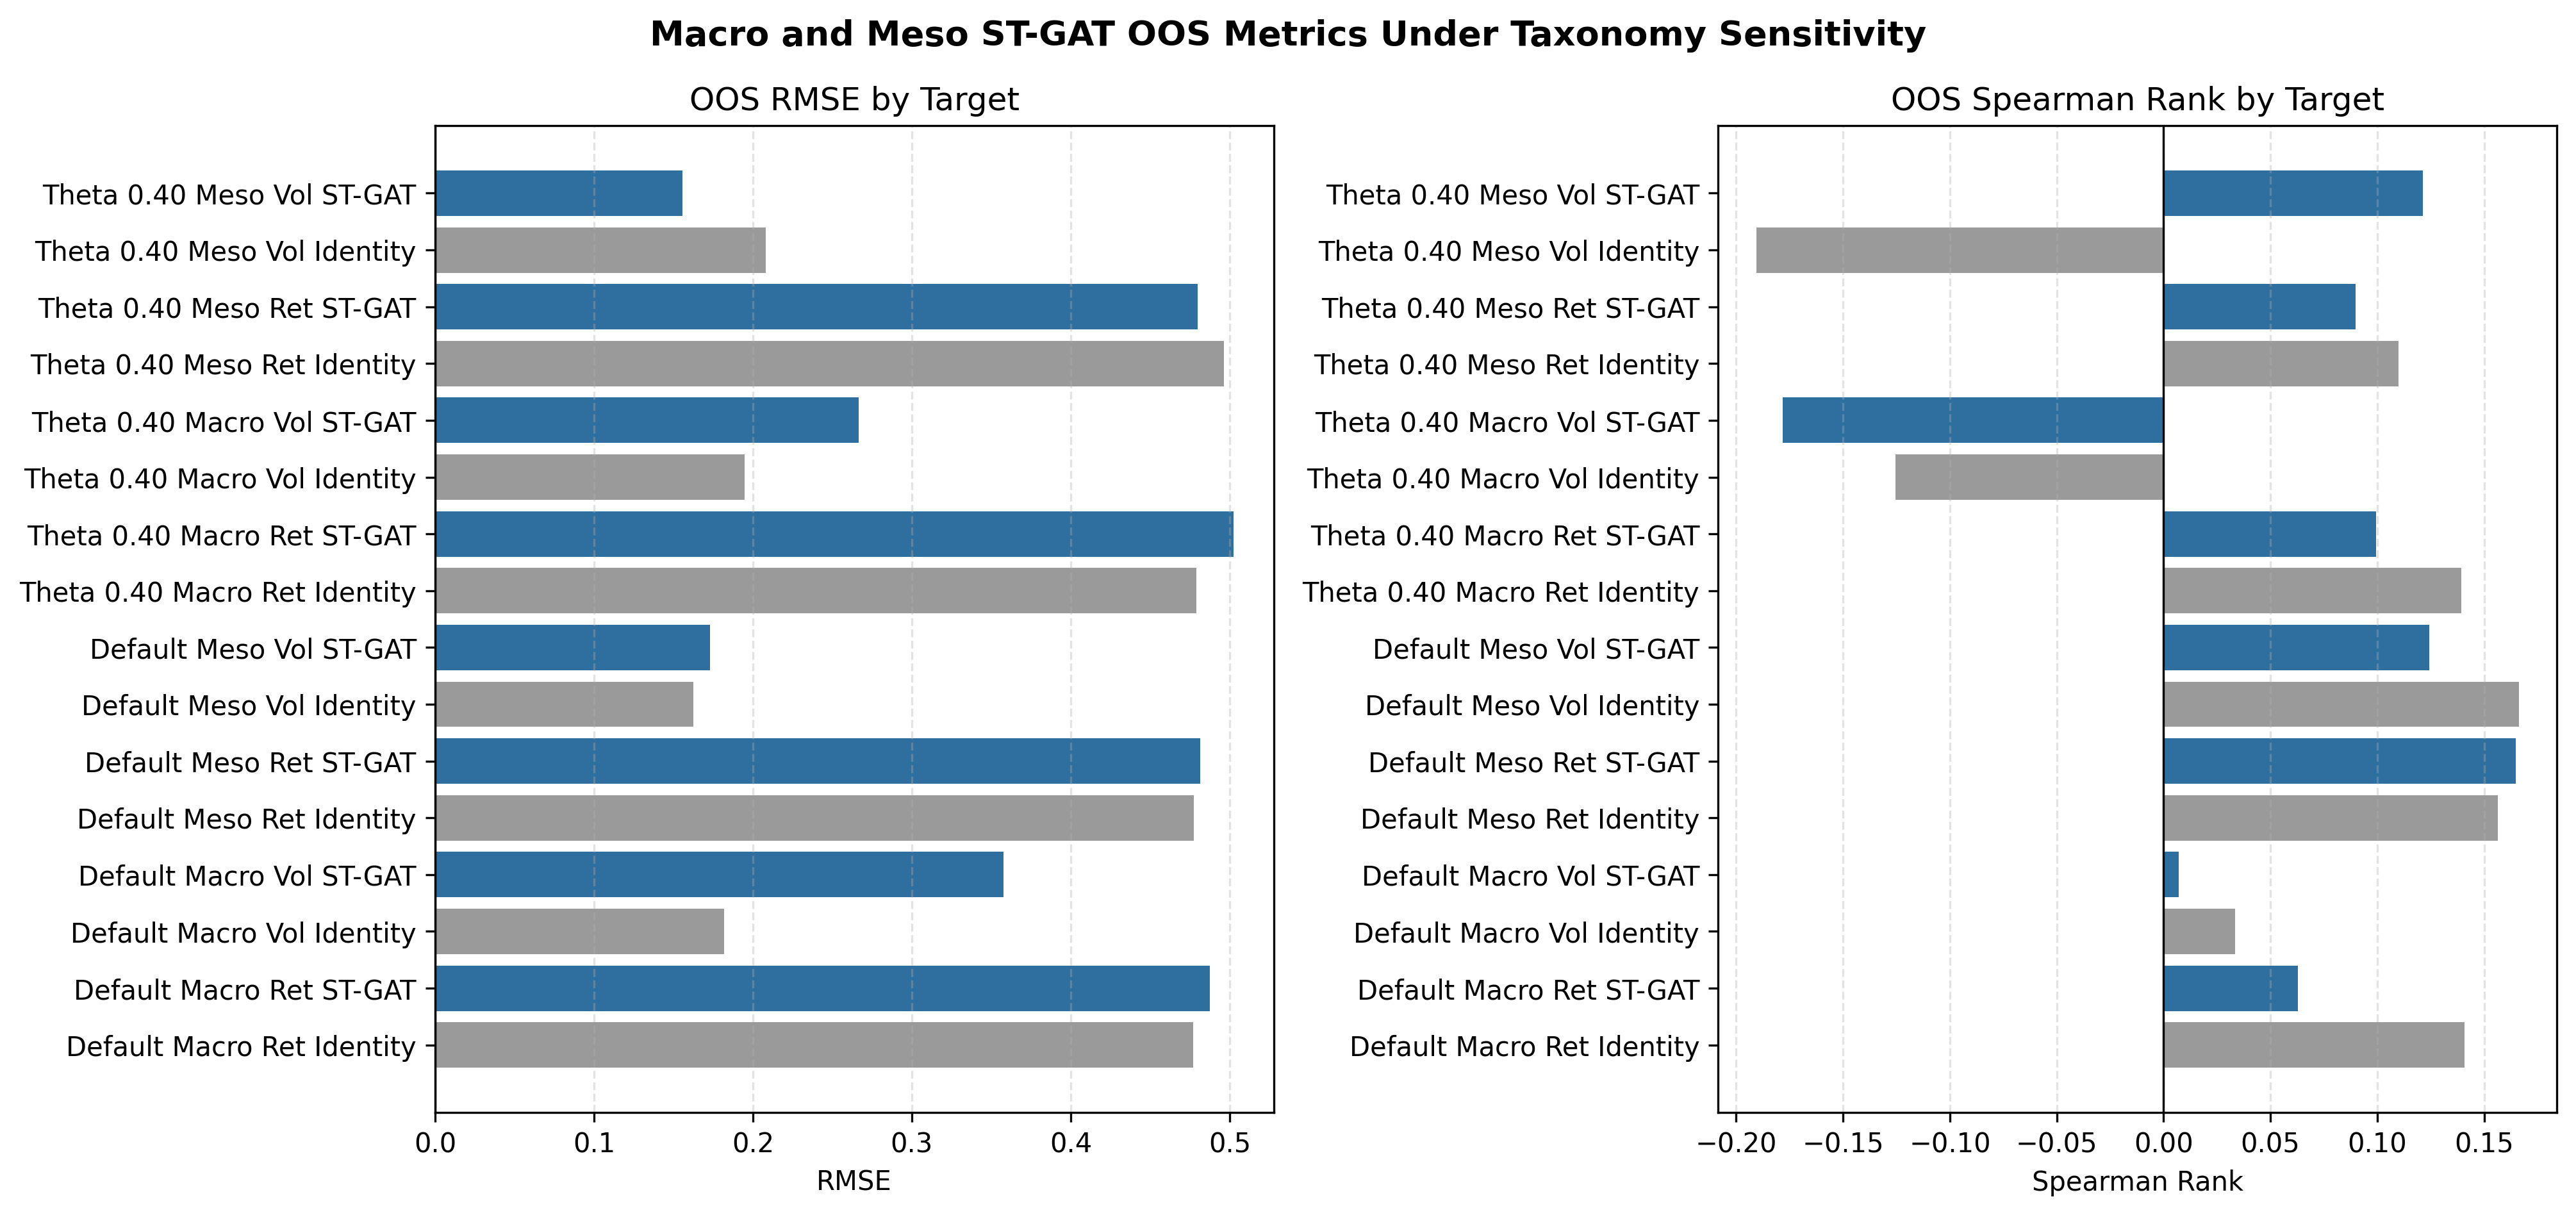
\includegraphics[width=0.92\linewidth]{oos_metric_comparison.png}
    \caption*{\textbf{OOS forecasting comparison.} The report compares
    Macro and Meso default and \texttt{theta040} outputs against matched
    identity baselines.}
\end{figure}

\section*{Graph Interpretation}

Graph-density diagnostics support the interpretation that taxonomy sensitivity
matters. During the OOS period, the default Meso graph retains 32--96
off-diagonal directed edges per year. The \texttt{theta040} Meso graph retains
100--630 edges and is materially denser in 2021, while Macro graphs retain
tens of thousands of links and become overconnected.

The report therefore frames the graph result as conditional evidence: taxonomy
settings alter graph density, forecast behavior, and portfolio ranking.

\begin{figure}[!htbp]
    \centering
    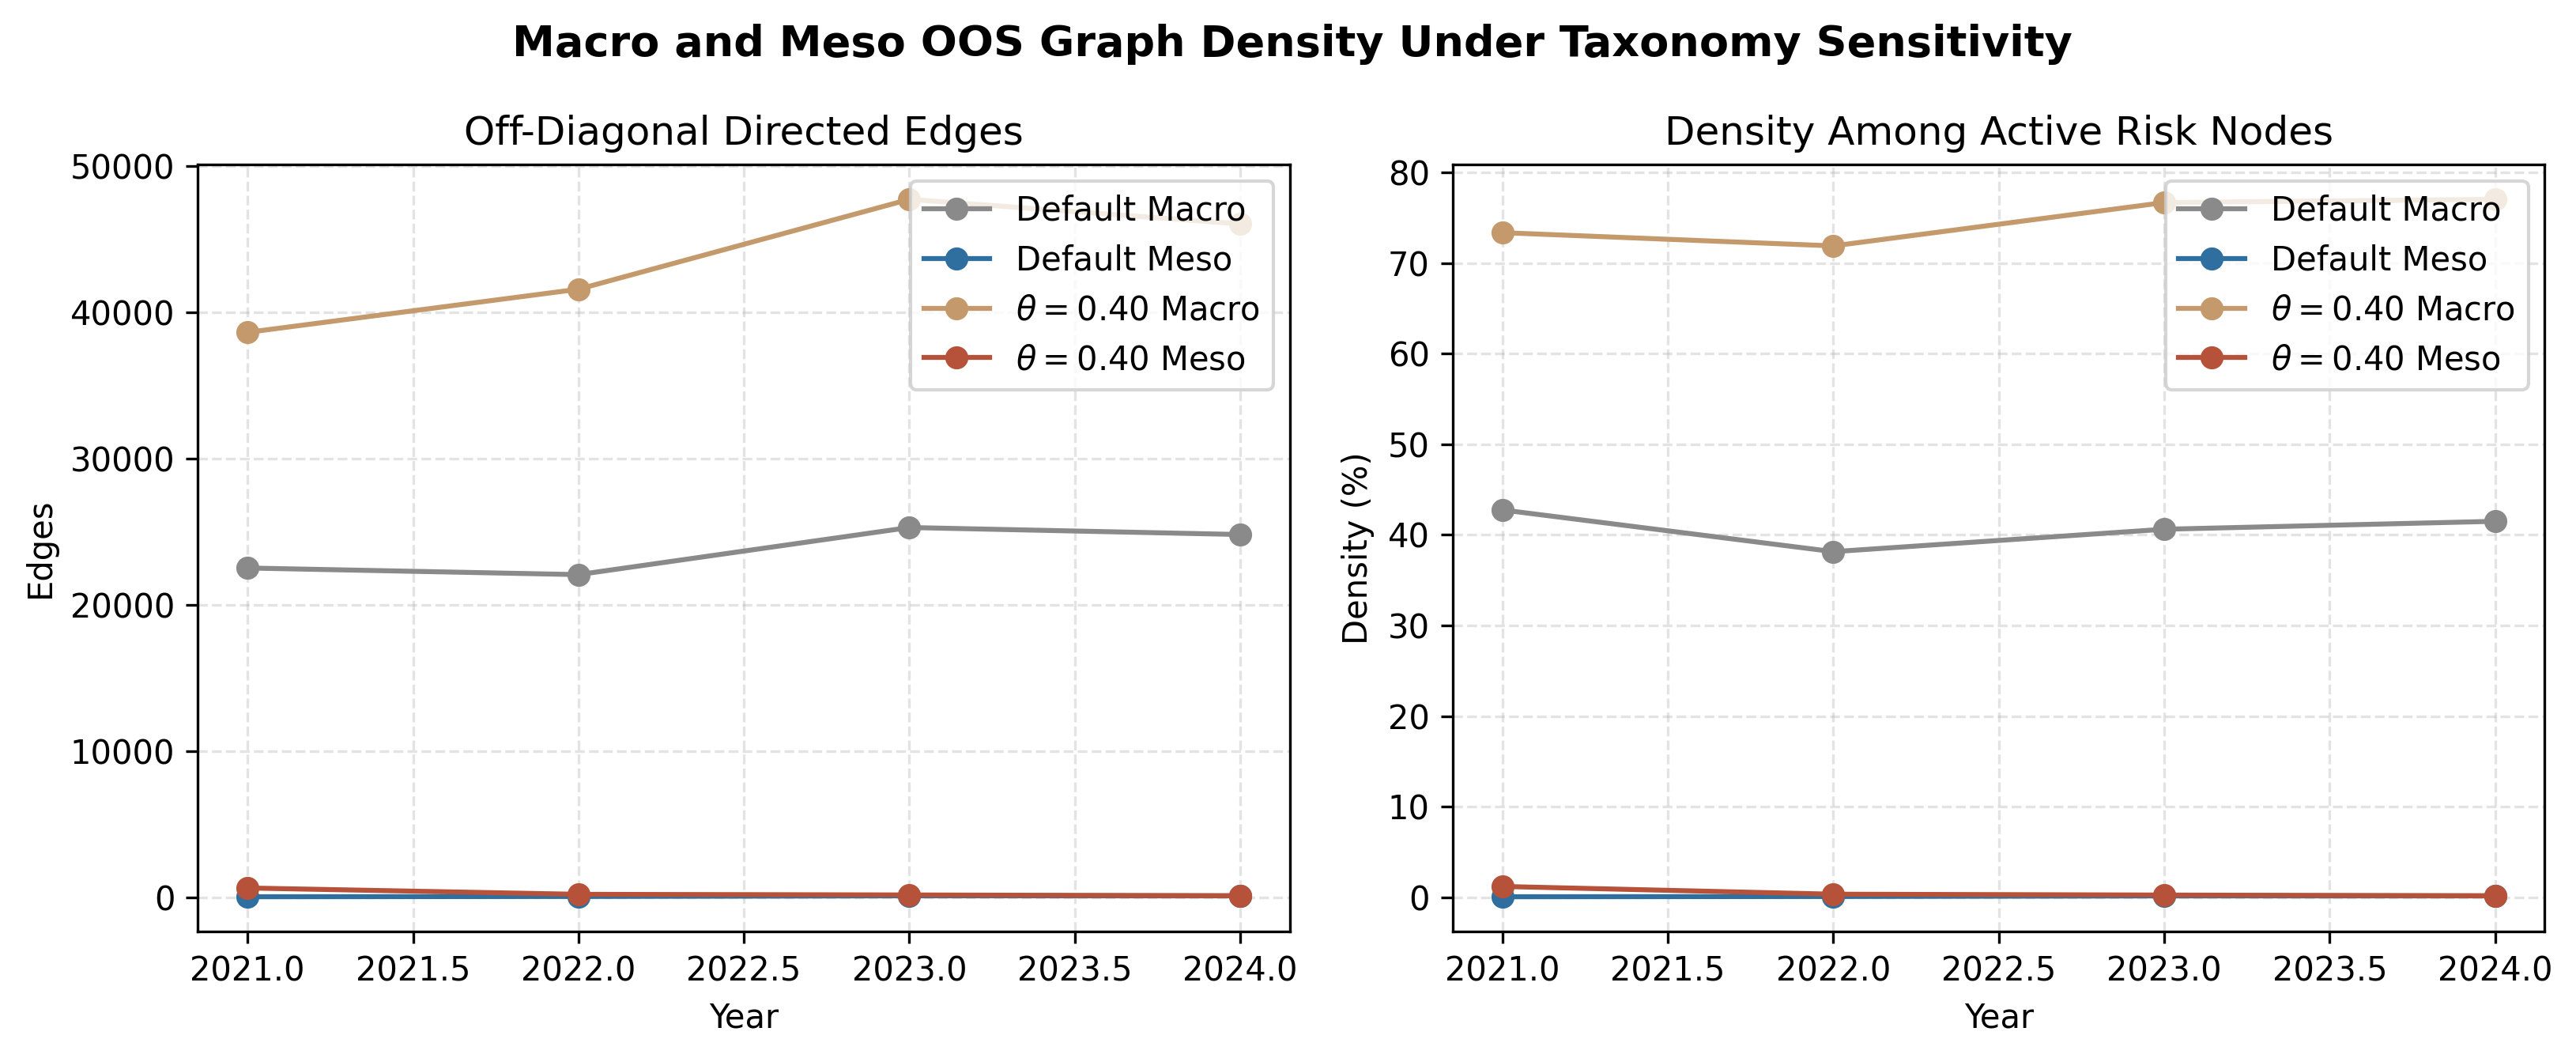
\includegraphics[width=0.88\linewidth]{graph_density_macro_meso.png}
    \caption*{\textbf{Graph-density diagnostic.} Macro and Meso taxonomies
    produce very different OOS graph densities.}
\end{figure}

\section*{Portfolio Validation}

The portfolio extension is presented as academic validation, not as live-trading
evidence. Annual Meso ST-GAT forecasts are held fixed over their July-to-June
forecast window, while portfolios are rebalanced monthly with 10 bps transaction
costs, 5 bps slippage, and SPY as benchmark.

The strongest return-only long-short strategy reports:

\begin{center}
\begin{tabular}{@{}ll@{}}
\toprule
Measure & Value \\
\midrule
Annualized return & 7.31\% \\
Annualized volatility & 8.34\% \\
Sharpe ratio & 0.88 \\
Sortino ratio & 1.52 \\
Maximum drawdown & -8.06\% \\
Beta versus SPY & 0.30 \\
Top-minus-bottom spread & 16.26\% annualized \\
Nominal spread p-value & 0.080 \\
\bottomrule
\end{tabular}
\end{center}

\begin{center}
    \centering
    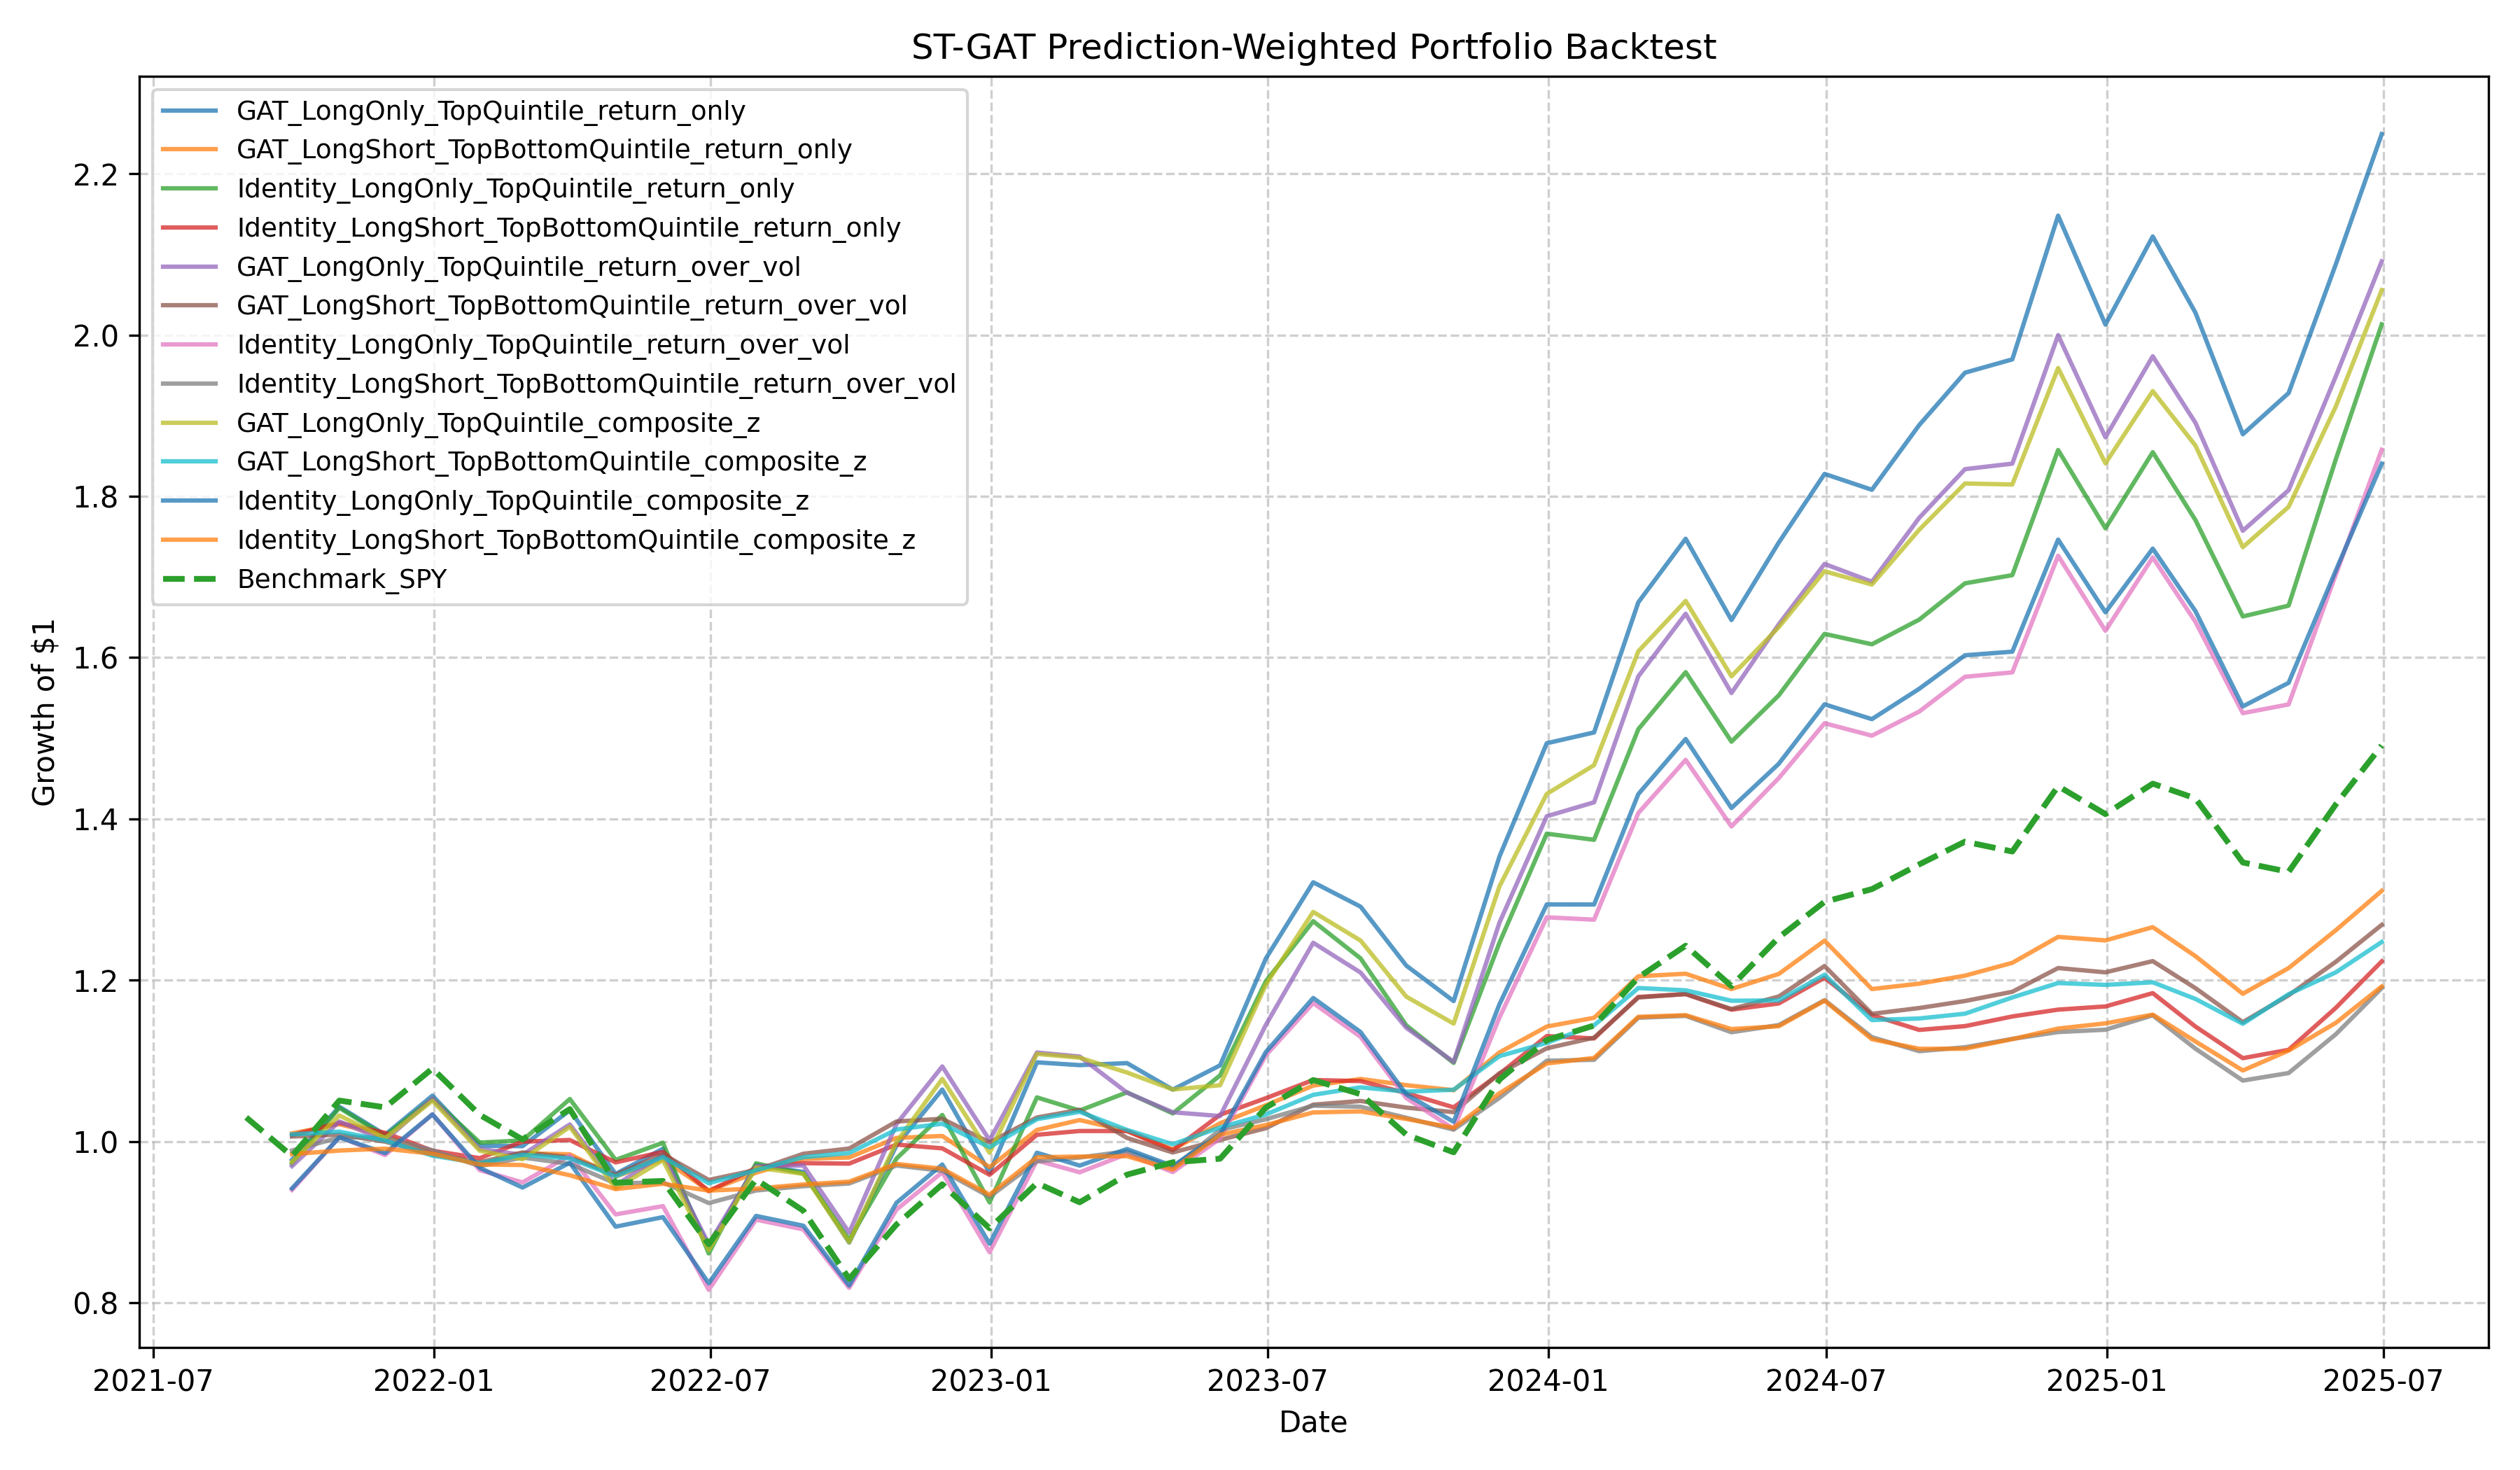
\includegraphics[width=0.96\linewidth]{portfolio_backtest_comparison.png}
    \captionof*{figure}{\textbf{Backtest comparison.} Monthly rebalanced ST-GAT and
    identity-baseline portfolio variants are compared against SPY using the
    current exported equity-curve artifact.}
\end{center}

The identity-baseline return-only signal has a smaller and insignificant
6.62\% annualized top-minus-bottom spread. This supports the interpretation
that semantic peer topology improves cross-sectional ranking quality, while the
report avoids presenting the result as investment advice or live-trading
deployability.

\begin{center}
    \centering
    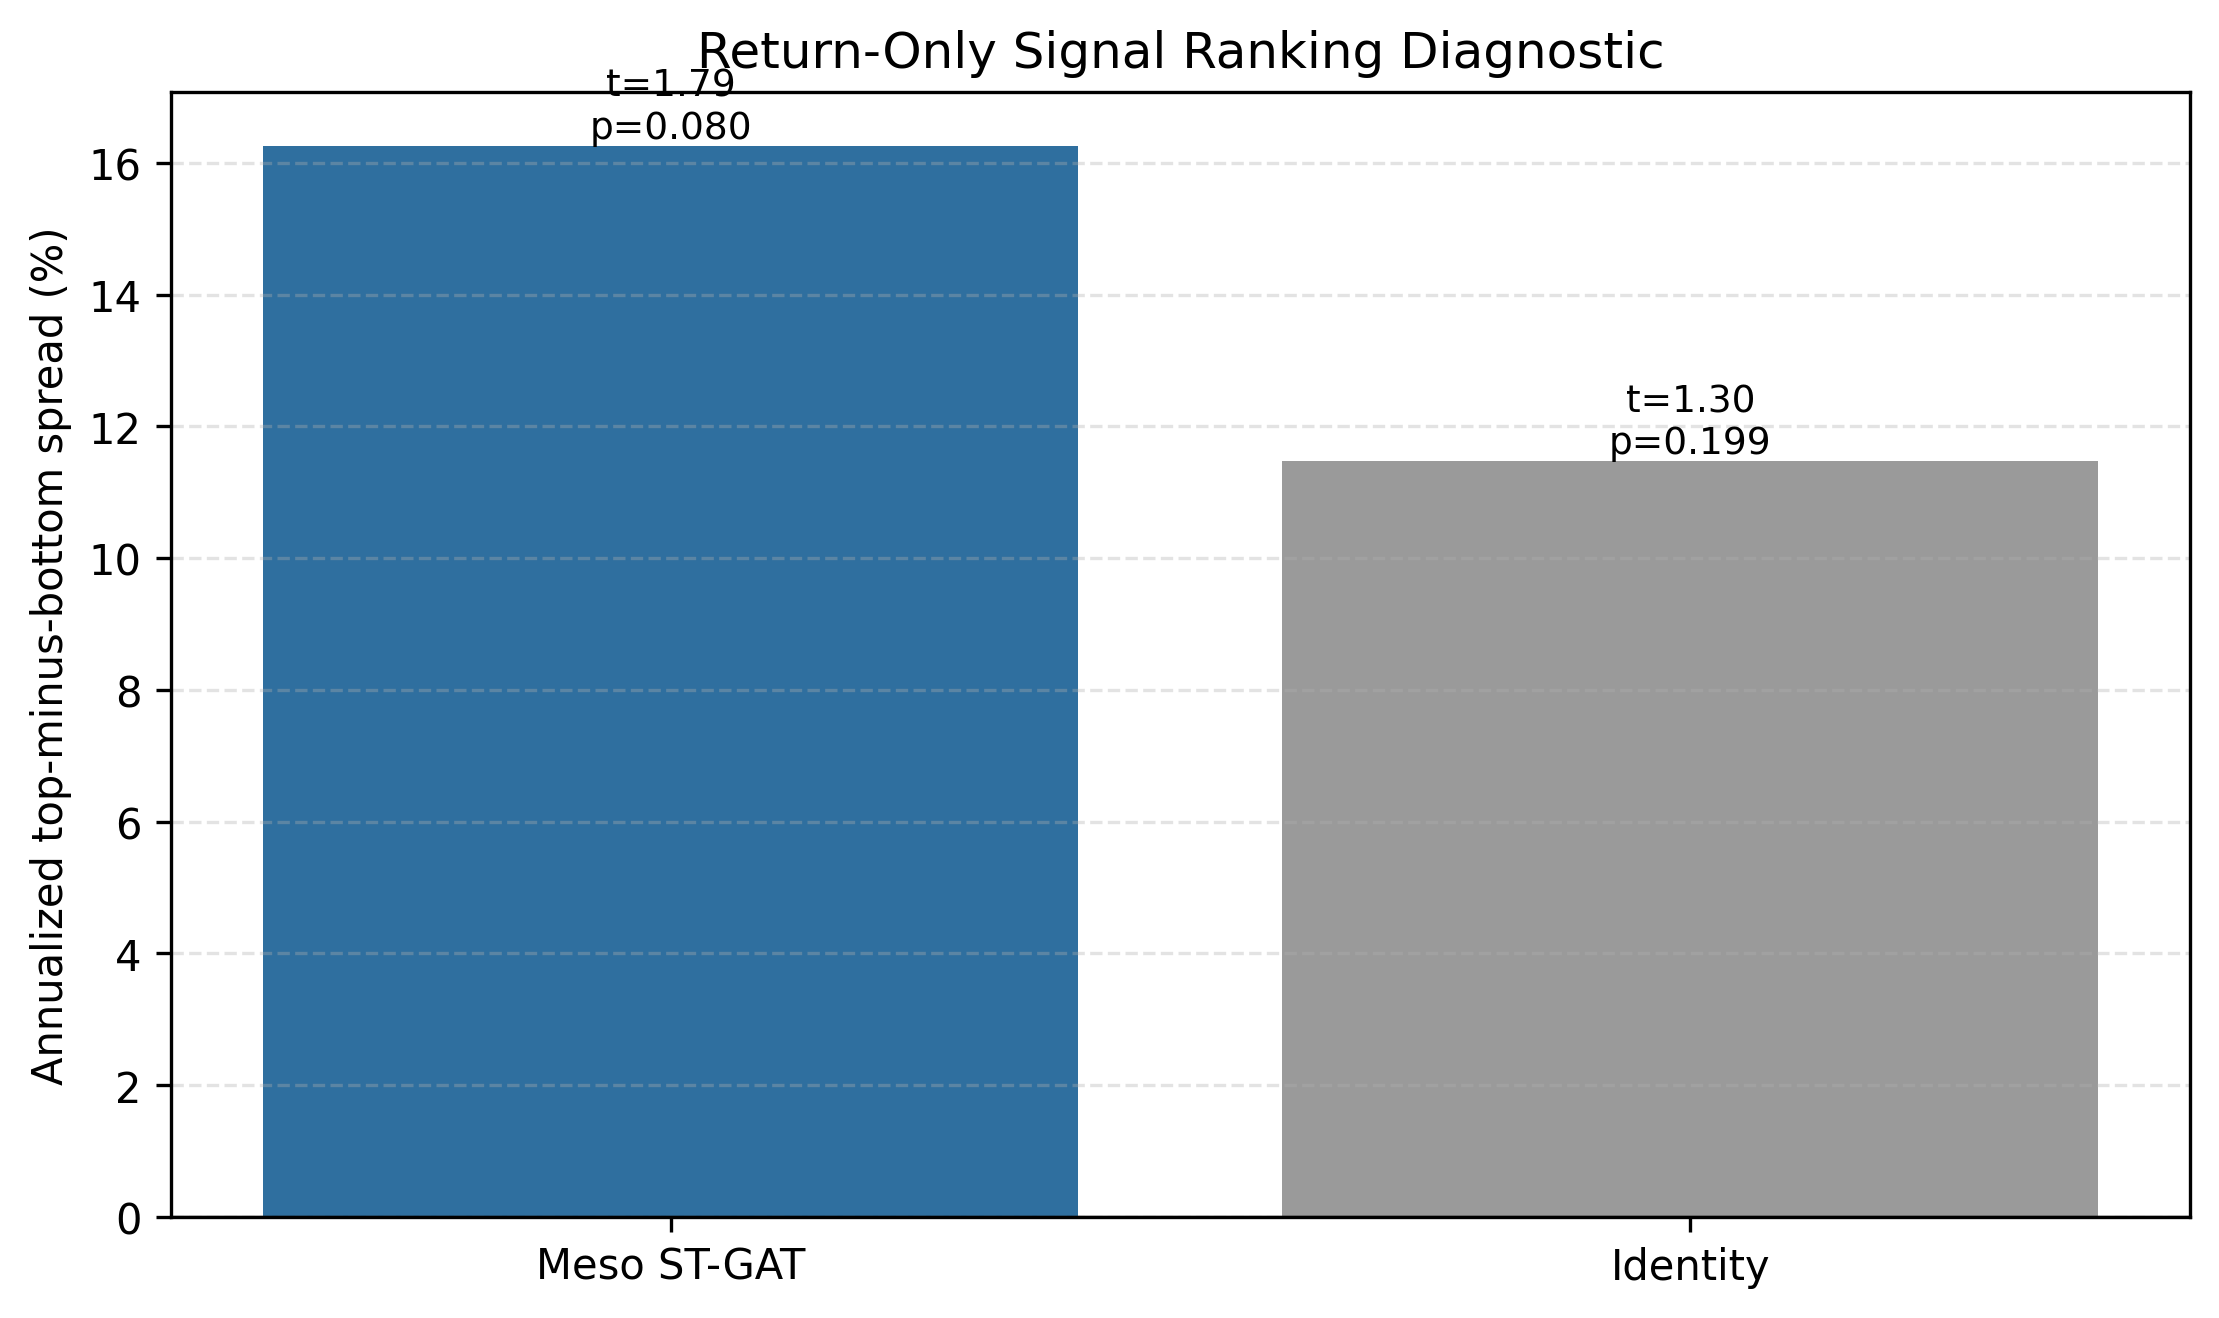
\includegraphics[width=0.82\linewidth]{portfolio_top_bottom_spread.png}
    \captionof*{figure}{\textbf{Portfolio ranking diagnostic.} The Meso ST-GAT return-only
    signal produces the strongest top-minus-bottom spread in the current
    academic backtest outputs.}
\end{center}

\section*{Claim Safety and Limitations}

The final package is deliberately conservative about unsupported evidence.
Old taxonomy-coverage percentages, unsupported single-firm migration claims,
DAV/EGARCH-X BIC comparisons, Fama-MacBeth tables, and SAR/network regression
claims are not used as headline findings unless their source tables are
regenerated and added to the output manifest. The updated taxonomy coverage and
case-study figures are backed by generated source CSVs and are interpreted as
taxonomy diagnostics, not standalone proof of forecast value.

The available DAV peak diagnostics are retained only as event-local context:
93 figures were parsed, with 20 positive improvements, 73 negative
improvements, and mean improvement of -2.40\%. These diagnostics do not
establish broad DAV dominance.

\section*{Repository Status}

Before GitHub cleanup, the complete local artifact set passed the lightweight
validation suite with 35 passes, 7 warnings, and 0 failures as of 2026-05-03.
The warnings are artifact-scope and research caveats rather than code crashes:
optional multi-seed, DAV, and taxonomy-interim files are absent from the
lightweight package; four financial feature values require downstream
train-period median imputation; and risk-year 2024 has a forward target window
ending on 2026-06-30.

The committed GitHub repository is a lightweight code, report, presentation,
and documentation package. Large raw data, intermediate files, generated
outputs, logs, and the local virtual environment are excluded from version
control and preserved outside the repository as local artifacts.

\end{document}
